%********************************************************************
% Appendix
%*******************************************************
% If problems with the headers: get headings in appendix etc. right
%\markboth{\spacedlowsmallcaps{Appendix}}{\spacedlowsmallcaps{Appendix}}
\chapter{Apéndice}

\section{Prueba de la identidad}\label{A:proof}
$$ S = \sum_{k=1}^n\cos{kx}=\cos{\frac{(n+1)x}{2}} \frac{\sin{\frac{nx}{2}}}{\sin{\frac{x}{2}}} $$

Dado que
\begin{equation}
  \label{eq:a.1}
  \exp{inx} = \cos{kx} + i \sin{kx}
\end{equation}

la suma $S$ se puede expresar como:
\begin{align}
  \label{eq:a.2}
  S &= \mathbb{R} \left ( \sum_{k=1}^n \exp{ikx}   \right ) \\
  &= \mathbb{R} \left( \exp{ix} + \exp{2ix} + \dots + \exp{inx} \right)
\end{align}

donde $\mathbb{R}$ representa la parte real. Reescribiendo cada término:

\begin{align}
  \label{eq:a.3}
  S  &= \mathbb{R} ( \exp{ix}\cdot 1 + \exp{ix} \cdot \exp{ix} + \exp{ix} \cdot \exp{2ix} \nonumber \\
  & + \dots + \exp{ix} \cdot \exp{(n-1)ix}) \nonumber \\
&= \sum_{k=0}^{n-1}\exp{ix} \cdot \left( \exp{ix} \right)^k
\end{align}

esta última expresión corresponde a una serie geométrica:

\begin{equation}
  \label{eq:a.4}
  \sum_{k=0}^{n-1} a \cdot r^k = \sum_{k=1}^n a \cdot r^{k-1} = a\left( \frac{r^n -1}{r-1}\right)
\end{equation}

con $a = r = \exp{ix}$, de esta manera el resultado de la suma es:

\begin{align}
  \label{eq:a.5}
  S & = \mathbb{R}\left ( \exp{ix}\frac{\exp{ixn}-1}{\exp{ix}-1}\right) \nonumber \\
  & = \mathbb{R} \left( \exp{ix} \frac{\exp{\frac{ixn}{2}}( \exp{\frac{ixn}{2}} - \exp{-\frac{ixn}{2}} )}{\exp{\frac{ix}{2}}( \exp{\frac{ix}{2}} - \exp{-\frac{ix}{2}} )} \right)
\end{align}

dado que:
\begin{equation*}
  \exp{-ik \theta} = \cos{k \theta} - i\sin{k \theta}
\end{equation*}
\begin{equation*}
  \Longrightarrow \exp{ik \theta} - \exp{-ik \theta} = 2i\sin{k \theta}
\end{equation*}

sustituyendo en la \autoref{eq:a.5}:

\begin{align}
  \label{eq:a.66}
  S &= \mathbb{R} \left( \frac{\exp{ix} \exp{\frac{inx}{2}}}{\exp{\frac{ix}{2}}} \cdot
      \frac{2i \sin{\frac{nx}{2}}}{2i\sin{\frac{x}{2}}} \right) \nonumber\\
  &= \mathbb{R} \left( \frac{\exp{ix} \exp{\frac{inx}{2}}}{\exp{\frac{ix}{2}}} \cdot
    \frac{\sin{\frac{nx}{2}}}{\sin{\frac{x}{2}}} \right) \nonumber\\
    & = \mathbb{R}\left( \exp{\frac{i(n+1)x}{2}} \frac{\sin{\frac{nx}{2}}}{\sin{\frac{x}{2}}} \right)\nonumber\\
  & = \cos{\frac{(n+1)x}{2}}\left(\frac{\sin{\frac{nx}{2}}}{\sin{\frac{x}{2}}} \right)
\end{align}

como se quería probar.























\section{Variables de parámetros para el potencial}

\begin{table}[H]
  \myfloatalign
  \begin{tabularx}{0.5\textwidth}{Xl} \toprule
   \tableheadline{Variable} & \tableheadline{Valor}\\ \midrule
    $V$          & 0.015936 $[a.u]$     \\ \midrule
    $\omega_1$   & 0.0110287 $[a.u]$   \\ \midrule
    $\omega_2$   & 0.0141751 $[a.u]$   \\ \midrule
    $\lambda$    & 0.00755816 $[a.u]$  \\ \midrule
    $X_{eq}$     & 0.00891848 $[a.u]$  \\ \midrule
    $\omega_x$   & 0.000357994 $[Jiffy^{-1}]$ \\ \midrule
    $\theta_X$   & 5.7759 $[rad]$   \\ \midrule
    $R_{eq}$     & 1.51438 $[a_0]$     \\ \midrule
    $R_0$        & 1.17396 $[a_0]$     \\ \midrule
    $\omega_{R}$ & 0.00103848 $[au]$   \\ \midrule
    $\theta_{R}$ & 0.429406 $[rad]$    \\ \midrule
    $m$          & 1836 $[m_e]$       \\
    \bottomrule
  \end{tabularx}
  \caption{Valores de parámetros del potencial utilizados para generar la gráfica de la \autoref{fig:drawPot}}
  \label{tab:ValuesPlot1}
\end{table}


\begin{table}[H]
  \myfloatalign
  \begin{tabularx}{0.5\textwidth}{Xl} \toprule
   \tableheadline{Variable} & \tableheadline{Valor}\\ \midrule
    $V$          & 0.015936 $[a.u]$     \\ \midrule
    $\omega_1$   & 0.006834 -- 0.018224 $[a.u.]$   \\ \midrule
    $\omega_2$   & 0.006834 -- 0.018224 $[a.u.]$   \\ \midrule
    $\lambda$    & 0 -- 0.015936 $[a.u]$  \\ \midrule
    $X_{eq}$     & -0.015936 -- 0.015936 $[a.u.]$  \\ \midrule
    $\omega_x$   & 0.000357994 $[Jiffy^{-1}]$ \\ \midrule
    $\theta_X$   & 0 -- 2$\pi$ $[rad]$   \\ \midrule
    $R_{eq}$     & 0.377945 -- 1.889725 $[a_0]$     \\ \midrule
    $R_0$        & 0 -- 2$R_{eq}$ $[a_0]$     \\ \midrule
    $\omega_{R}$ & 0.0004556 -- 0.0013668 $[a.u.]$   \\ \midrule
    $\theta_{R}$ & 0 -- 2$\pi$ $[rad]$    \\ \midrule
    $m$          & 1836 $[m_e]$       \\
    \bottomrule
  \end{tabularx}
  \caption{Rango de valores de parámetros del potencial utilizados para generar trayectorias.}
  \label{tab:RangeValuesPot}
\end{table}

\section{Ejemplos de potenciales utilizados}

\begin{figure}[H]
  \centering
  \makebox[\textwidth][c]{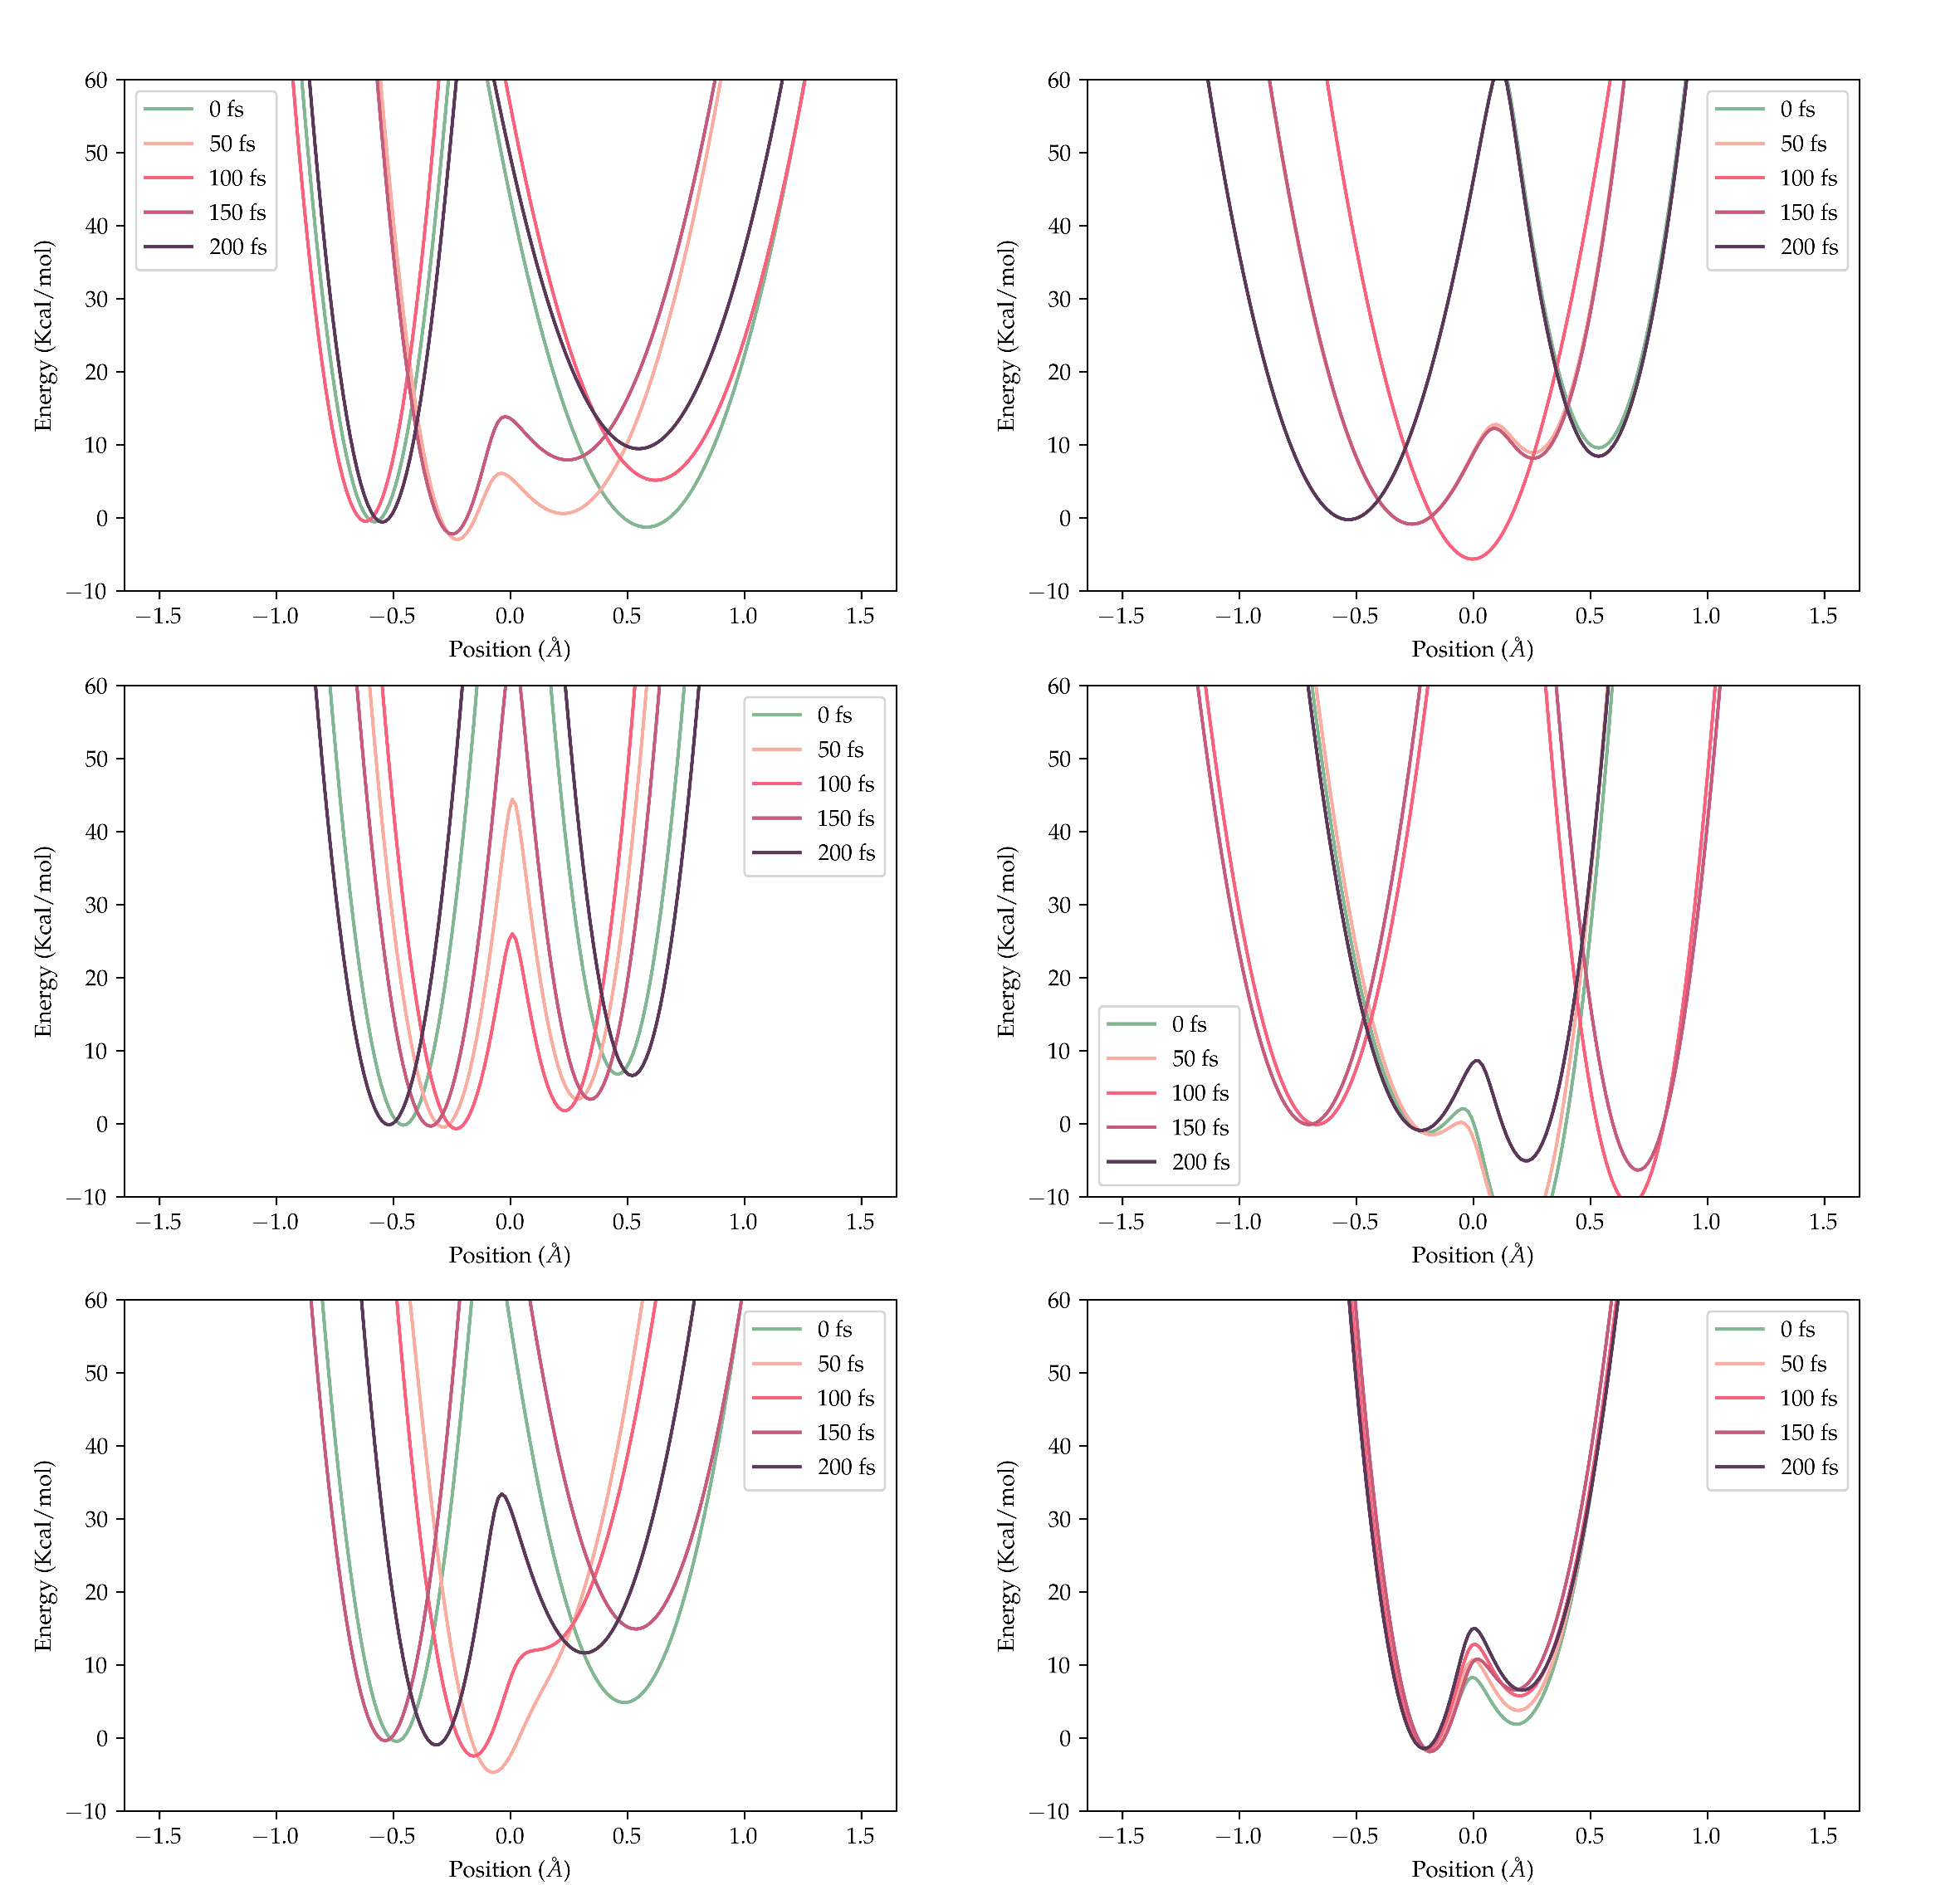
\includegraphics[width=1.4\textwidth]{/home/jessica/Tesis/img/tesis/ExamplesPotentialApen.png}}
  \caption{Ejemplos de potenciales utilizados $V(r,t)$}
  %\label{fig:dens_ev}
\end{figure}

\begin{figure}[H]
  \centering
  \makebox[\textwidth][c]{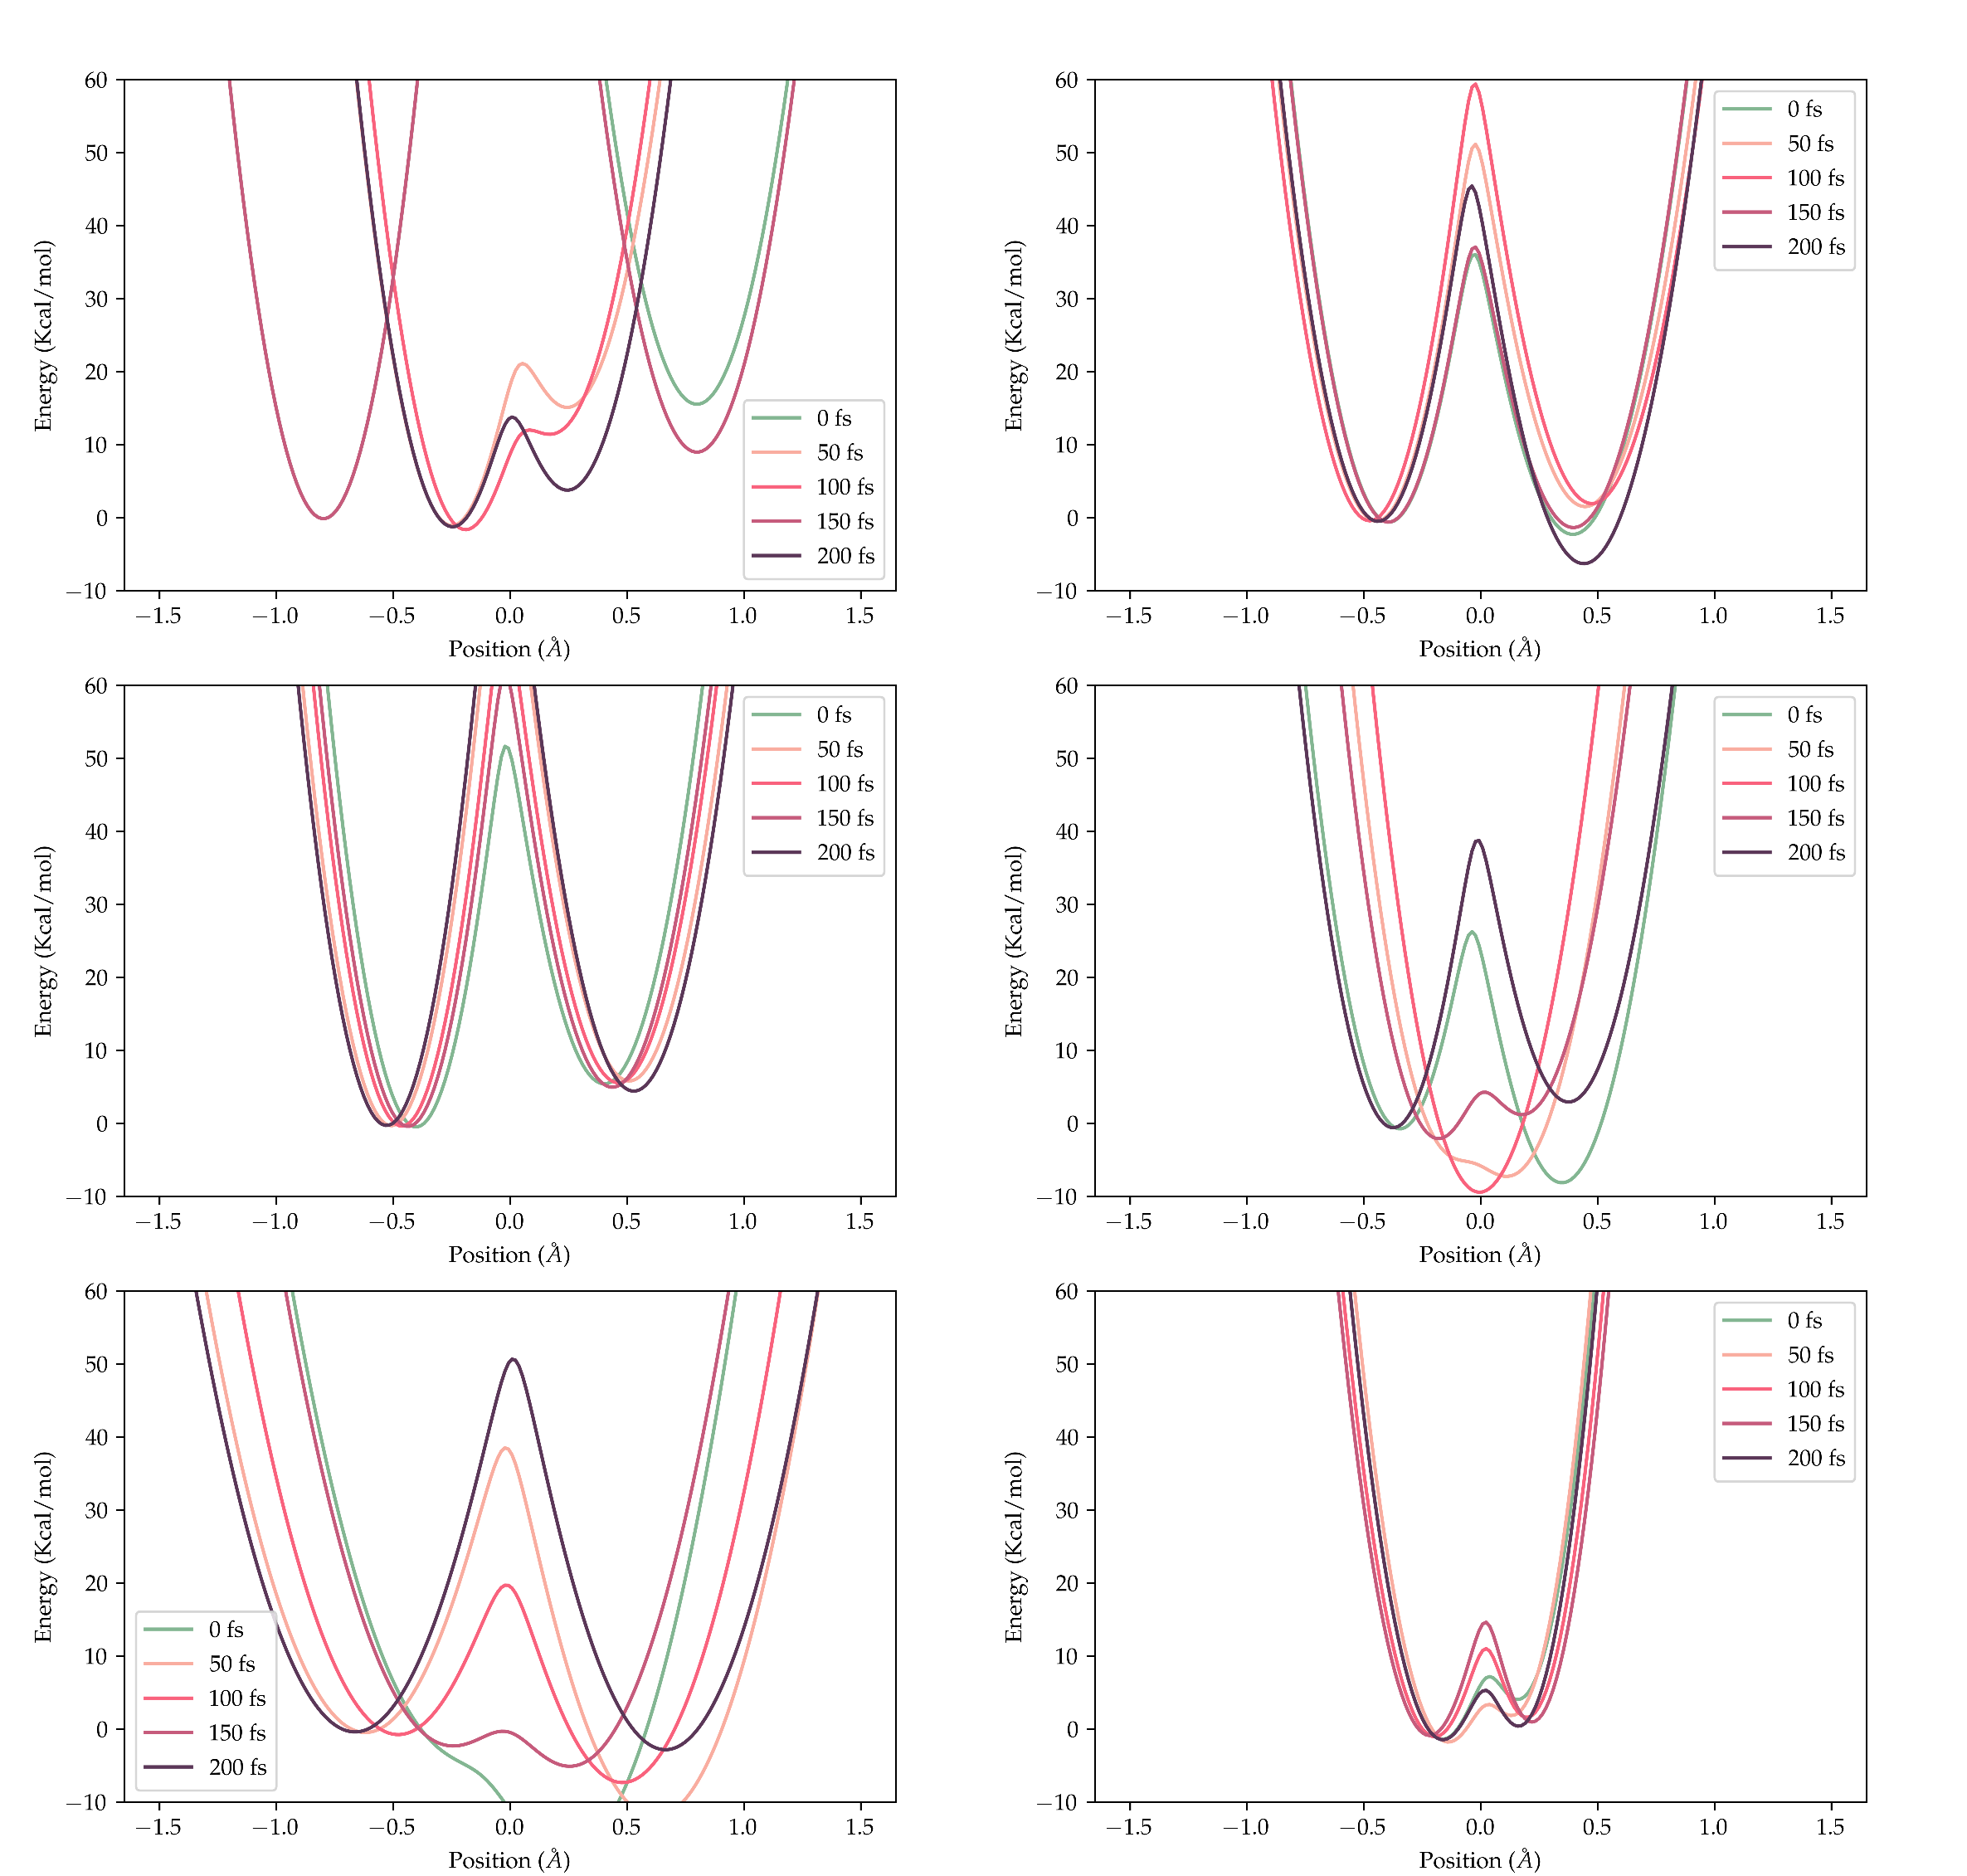
\includegraphics[width=1.4\textwidth]{/home/jessica/Tesis/img/tesis/ExamplesPotentialApen1.png}}
  \caption{Ejemplos de potenciales utilizados $V(r,t)$}
  %\label{fig:dens_ev}
\end{figure}




\section{Unidades atómicas (a.u.)}
%\faHandshake[regular] No pelien
%------------ Tabla 1 unidades atómicas
%----------------------------------------------
\begin{table}[H]
  \myfloatalign
  \begin{tabularx}{\textwidth}{Xll} \toprule
   \tableheadline{Unidades Atómicas} & \tableheadline{Valor SI} & \tableheadline{Nombre (símbolo)}\\ \midrule
    Masa $m_e$                  & 9.10939(-31)  & Masa del electrón     \\ \midrule
    Carga $e$                   & 1.602188(-19) & Carga del electrón \\ \midrule
    Momento angular $\hbar$     & 1.05457(-34) & Constante de Planck$/2\pi$   \\ \midrule
    Energía $(m_e e^4/\hbar^2)$  & 4.35975(-18)  & Hartree $(H)$\\ \midrule
    Longitud $(\hbar^2/m_ee^2)$  & 5.29177(-11)  & Radio de Bohr $(a_0)$\\ \midrule
    Tiempo $(\hbar^3/m_ee^4)$    & 2.41888(-17)  & Jiffy \\ \midrule
    {Momento Dipolar Eléctrico} $(\hbar^2/m_ee)$ & 8.47836(-30) & 2.541765 Debye $(D)$units  \\ \midrule
    Momento Dipolar Magnético $(e\hbar/2m_e)$  & 9.27402(-24)    & Magneton de Bohr $(\mu_B)$    \\
    \bottomrule
  \end{tabularx}
  \caption{Conversión de unidades atómicas a unidades SI.}
  \label{tab:AU-SI}
\end{table}
%------------ Tabla 2 unidades atómicas Energía
%----------------------------------------------

\begin{table}[H]
  \myfloatalign
  % \resizebox{0.5\textwidth}{!}{%
  \footnotesize
  \begin{tabularx}{\textwidth}{XXXXXX} \toprule
   Unidad      & $a.u.$ & $kcal/mol$  & $eV$        & $cm^{-1}$    & $Hz$        \\ \midrule% & $K$          \\ \midrule
    $a.u.$     & 1      & 6.27510(2) & 2.72114(1) & 2.19475(5) & 6.57968(15) \\ \midrule%& 3.15773 (5)  \\ \midrule
    $kcal/mol$ & 1.59360(-3) & 1     & 4.33641(-2)& 3.49755(2) & 1.04854(13) \\ \midrule%& 5.03217 (2)  \\ \midrule
    $eV$       & 3.67493(-2) & 2.30605(1) & 1     & 8.06554(3) & 2.41799(14) \\ \midrule%& 1.16044 (4)  \\ \midrule
    $cm^{-1}$   & 4.55634(-6) & 2.85914(-3) & 1.23984(-4) & 1   & 2.99792(10) \\ \midrule%& 1.43877      \\ \midrule
    $Hz$       & 1.51983(-16)& 9.5371(-14) & 4.13567(-15) & 3.33564(-11) & 1  \\ %\midrule& 4.79922 (-11)\\ %\midrule
   % $K$        & 3.16683 (-6) & 1.98722 (-3) & 8.61739 (-5) & 6.95039 (-1) & 2.08367 (10)& 1   \\ 
    \bottomrule
  \end{tabularx}%}
  \caption{Conversión de energía (diversas unidades).}
  \label{tab:AU-SI}
\end{table}









%\begin{lstlisting}[float=b,language=Pascal,frame=tb,caption={A floating example (\texttt{listings} manual)},label=lst:useless]
%for i:=maxint downto 0 do
%begin
%{ do nothing }
%end;
%\end{lstlisting}

%Ei solet nemore consectetuer nam. Ad eam porro impetus, te choro omnes
%evertitur mel. Molestie conclusionemque vel at, no qui omittam
%expetenda efficiendi. Eu quo nobis offendit, verterem scriptorem ne
%vix.

